%%%%%%%%%%%%%%%%%%%%%%%%%%%%%%%%%%%%%%%%%%%%%%%%%%%%%%%%%%%%%%%%%%%%%%%%%%%
%% This file is part of the book
%%
%% Algorithmic Graph Theory
%% http://code.google.com/p/graph-theory-algorithms-book/
%%
%% Copyright (C) 2009, 2010, 2011 Minh Van Nguyen <nguyenminh2@gmail.com>
%%
%% See the file COPYING for copying conditions.
%%%%%%%%%%%%%%%%%%%%%%%%%%%%%%%%%%%%%%%%%%%%%%%%%%%%%%%%%%%%%%%%%%%%%%%%%%%

\documentclass{article}

\usepackage{subfigure}
\usepackage{tikz}
\usetikzlibrary{external}
\tikzexternalize{five-complete-graphs}

\begin{document}

\begin{figure}
%% complete graph K_5
\subfigure[$K_5$]{
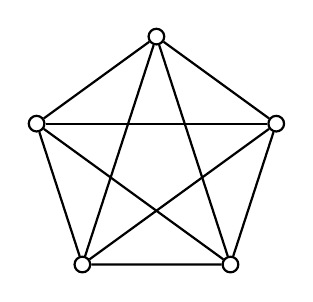
\begin{tikzpicture}
[nodeDecorate/.style={shape=circle,inner sep=2pt,draw,thick},%
  lineDecorate/.style={-,thick},%
  scale=1.6]
%% nodes or vertices
\foreach \nodename/\x/\y in {
  1/0.9510/0.3090, 2/0/1, 3/-0.9510/0.3090, 4/-0.5877/-0.8090,
  5/0.5877/-0.8090}
{
  \node (\nodename) at (\x,\y) [nodeDecorate] {};
}
%% edges or lines
\path
\foreach \startnode/\endnode in {
  1/2, 1/3, 1/4, 1/5, 2/3, 2/4, 2/5, 3/4, 3/5, 4/5}
{
  (\startnode) edge[lineDecorate] node {} (\endnode)
};
\end{tikzpicture}
}
%%
%%
\quad
%% complete graph K_4
\subfigure[$K_4$]{
\label{fig:five_complete_graphs:complete_graph_on_four_vertices}
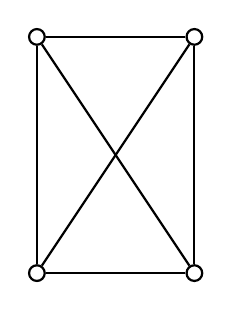
\begin{tikzpicture}
[nodeDecorate/.style={shape=circle,inner sep=2pt,draw,thick},%
  lineDecorate/.style={-,thick}]
%% nodes or vertices
\foreach \nodename/\x/\y in {1/0/0, 2/2/0, 3/2/3, 4/0/3}
{
  \node (\nodename) at (\x,\y) [nodeDecorate] {};
}
%% edges or lines
\path
\foreach \startnode/\endnode in {1/1, 1/2, 1/3, 1/4, 2/3, 2/4, 3/4}
{
  (\startnode) edge[lineDecorate] node {} (\endnode)
};
\end{tikzpicture}
}
%%
%%
\quad
%% complete graph K_3
\subfigure[$K_3$]{
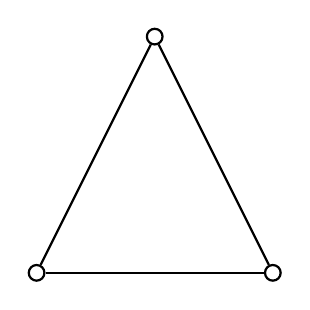
\begin{tikzpicture}
[nodeDecorate/.style={shape=circle,inner sep=2pt,draw,thick},%
  lineDecorate/.style={-,thick}]
%% nodes or vertices
\foreach \nodename/\x/\y in {1/0/0, 2/3/0, 3/1.5/3}
{
  \node (\nodename) at (\x,\y) [nodeDecorate] {};
}
%% edges or lines
\path
\foreach \startnode/\endnode in {1/2, 1/3, 2/3}
{
  (\startnode) edge[lineDecorate] node {} (\endnode)
};
\end{tikzpicture}
}
%%
%%
\quad
%% complete graph K_2
\subfigure[$K_2$]{
\begin{tikzpicture}
[nodeDecorate/.style={shape=circle,inner sep=2pt,draw,thick},%
  lineDecorate/.style={-,thick}]
%% nodes or vertices
\node (1) at (0,0) [nodeDecorate] {};
\node (2) at (0,3) [nodeDecorate] {};
%% stub nodes that should not be visible
\node () at (-0.5,0) [] {};
\node () at (0.5,0) [] {};
%% edges or lines
\path
(1) edge[lineDecorate] node {} (2);
\end{tikzpicture}
}
%%
%%
\quad
%% complete graph K_1
\subfigure[$K_1$]{
\begin{tikzpicture}
[nodeDecorate/.style={shape=circle,inner sep=2pt,draw,thick}]
%% nodes or vertices
\node at (0,0) [nodeDecorate] {};
%% stub nodes that should not be visible
\node at (-0.5,0) {};
\node at (0.5,0) {};
\end{tikzpicture}
}
\end{figure}

\end{document}
